\chapter{Ausbaustufe 1}

\section{Dokumentation Ausbaustufe
1}\label{dokumentation-ausbaustufe-1}


\subsection{Datenbankmodell}\label{datenbankmodell}

\subsubsection{Station}\label{station}

Für die Stationen werden ein Name sowie der Längen- und Breitengrad gespeichert. Außerdem wird gespeichert, welcher Stationstyp die Station ist und in welcher Gemeinde sie sich befindet. Für jede Station wird der User gespeichert, der die Station erstellt hat.


\subsubsection{Stationstyp}\label{stationstyp}

Es werden die Hersteller und die Modelle der Stationen gespeichert.


\subsubsection{Bundesland, Bezirk,
Gemeinde}\label{bundesland-bezirk-gemeinde}

Für alle Elemente werden der Name und eine ID gespeichert. Für die
Bezirke wird gespeichert, in welchem Bundesland sie sich befinden. Für
Gemeinden wird der Bezirk in dem sie sich befinden, sowie die
Postleitzahl gespeichert.

\subsubsection{Benutzer}\label{benutzer}

Für Benutzer der Anwendung werden eine ID, der Username, das Password,
eine Email Adresse, der Vor- und Nachname und das Geburtsdatum
gespeichert. Außerdem wird die Gemeinde, in der sie wohnen, gespeichert.


\subsubsection{Einheit}\label{einheit}

Für jede Einheit wird ein Kürzel (z.B. °C), sowie der volle Name (z.B.
Grad Celsius) gespeichert.


\subsubsection{Messungstyp}\label{messungstyp}

Es wird der Name des Messungstyps (z.B. Temperatur, Luftdruck)
gespeichert.


\subsubsection{Messung}\label{messung}

Für jede Messung wird eine ID, der Wert der Messung und ein Timestamp
mit Datum und Uhrzeit gespeichert. Außerdem werden der Typ sowie die
Einheit der Messung und die Station, die die Messung durchgeführt hat,
gespeichert.

\begin{figure}[!htbp]
	\centering
	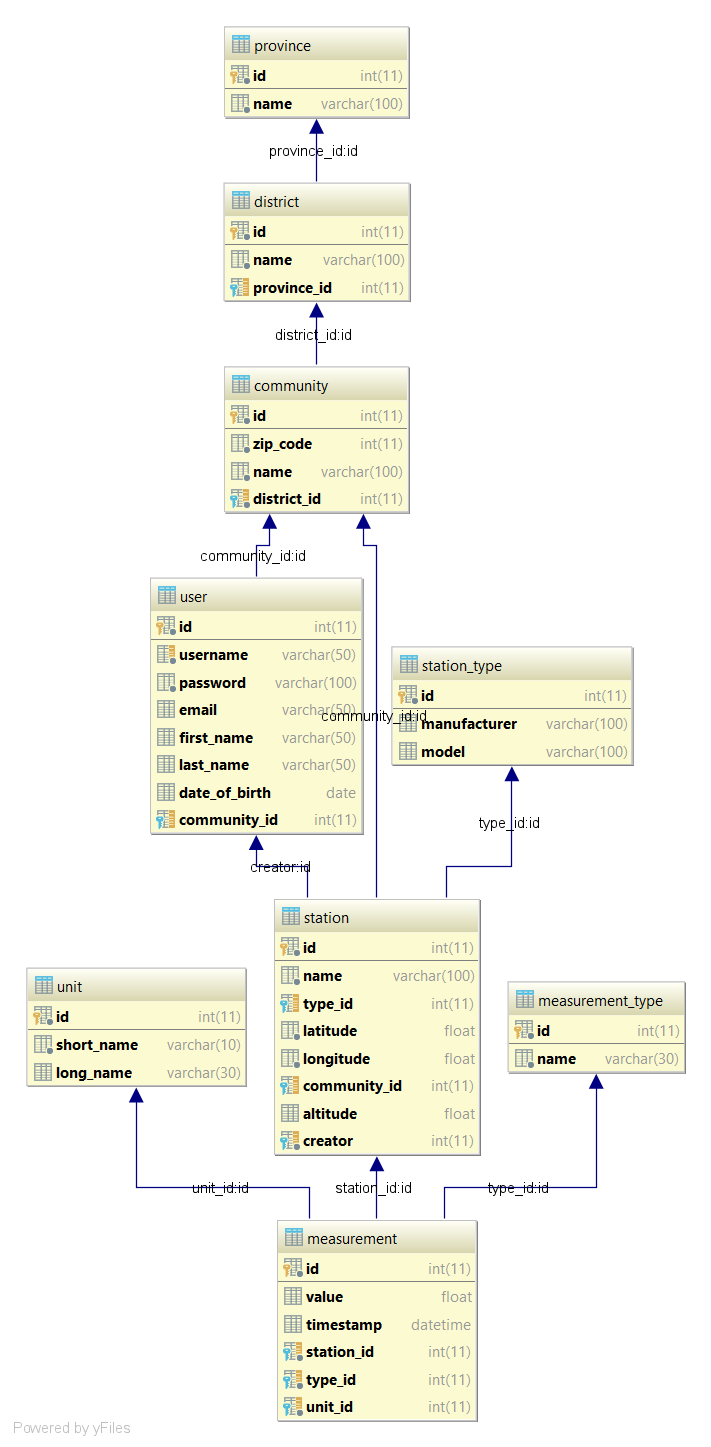
\includegraphics[width=0.6\textwidth]{WetrDB.png}
	\caption{UML Darstellung der Testdatenbank}
	\label{fig:WetrDB}
\end{figure}

\newpage

\subsection{Datenbankzugriffsschicht}\label{datenbankzugriffsschicht}

Der Aufbau der ersten Ausbaustufe wurde nach dem DAO Muster realisiert.
Es wurden Domänenklassen (Wetr.Server.Dal.Domain) mit Properties und
Konstruktoren erstellt. Diese Domänenklassen können in Folge dann auch
von der Geschäftslogik und bei der Implementierung der Interfaces für
die Datenbankzugriffe verwendet werden. Die Implementierung der
Interfaces wurde mit ADO.NET erstellt.


\subsubsection{Hilfsklassen(Dal.Common)}\label{hilfsklassendal.common}


\paragraph{DefaultConnectionFactory}\label{defaultconnectionfactory}

Um eine Datenbankverbindung herzustellen wird die Klasse
DefaultConnectionFactory verwendet, mithilfe dieser Klasse kann eine
Verbindung hergestellt werden, indem nur ein Konfigurationsname
angegeben werden muss. Es wird dann nach einem XML-Element mit diesem
Namen in der App.config Datei des jeweiligen Projekts gesucht, und der
ConnectionString und der ProviderName aus dieser Datei für die
Datenbankverbindung verwendet.


\paragraph{AdoTemplate}\label{adotemplate}

Die Klasse AdoTemplate stellt Methoden zur Verfügung, über die Abfragen
auf die Datenbank ausgeführt werden können. Das ist mit den
Query-Methoden möglich. Es können auch Anweisungen wie Insert, Update
oder Delete über die ExecuteStatement Methoden durchgeführt werden. Es
gibt für Query und ExecuteStatement jeweils synchrone und asynchrone
Varianten.


\paragraph{QueryParameter}\label{queryparameter}

Mit dieser Klasse können Parameter in SQL-Abfragen gesetzt werden. Die
Klasse speichert die Werte, die diese Parameter in der SQL Abfrage
ersetzten.


\paragraph{Delegates}\label{delegates}

In dieser Klasse werden notwendige Delegates für den Datenbankzugriff
definiert, momentan ist ein Delegate für das Mappen von Queryergebnissen
in ein Domainobjekt in der Klasse enthalten.

\paragraph{IConnectionFactory}\label{iconnectionfactory}

IConnectionFactory dient als Interface für die Erstellung einer
Datenbankverbindung. IConnectionFactory wird in diesem Projekt durch
DefaultConnectionFactory implementiert.


\subsubsection{Zugriffsklassen
(Wetr.Server.Dal.Ado)}\label{zugriffsklassen-wetr.server.dal.ado}

Funktionen für das Datenbankmodell wurden in Zugriffsklassen erstellt.
Damit die Implementierungen der Funktionen leicht austauschbar bleiben,
wurden die Zugriffsklassen in Interfaces definiert. Im Programm wird mit
Domänenobjekten gearbeitet. Jede Tabelle im Datenmodell wurde in einer
Domainklasse abgebildet.

Da der Datenbankzugriff etwas länger dauern kann, wurden alle Abfragen
asynchron implementiert.

In der Folgenden Auflistung ist zu erkennen, welche Zugriffsfunktionen
momentan für die jeweilige Datenbanktabelle im Interface definiert
wurden. Diese wurden durch eine ADO.net Klasse ausimplementiert.


\paragraph{AdoProvinceDao}\label{adoprovincedao}

Abfrage nach:

\begin{itemize}

\item
  allen Bundesländern
\item
  Bundesland mit bestimmter ID
\item
  Bundesland mit bestimmtem Namen
\end{itemize}

Zusätzlich einfügen, aktualisieren und löschen von Bundesländern mit
einem Bundeslandobjekt als Übergabeparameter.


\paragraph{AdoDistrictDao}\label{adodistrictdao}

Abfrage nach:

\begin{itemize}

\item
  allen Bezirken
\item
  Bezirken mit bestimmter ID
\item
  Bezirken mit bestimmtem Namen
\item
  Bezirke eines bestimmten Bundeslandes
\end{itemize}

Zusätzlich einfügen, aktualisieren und löschen von Bezirken mit einem
Bezirksobjekt als Übergabeparameter.


\paragraph{AdoCommunityDao}\label{adocommunitydao}

Abfrage nach:

\begin{itemize}

\item
  allen Gemeinden
\item
  Gemeinden mit bestimmter ID
\item
  Gemeinden mit bestimmtem Namen
\item
  Gemeinden mit bestimmtem Bezirk
\item
  Gemeinden mit bestimmter Postleitzahl
\end{itemize}

Zusätzlich einfügen, aktualisieren und löschen von Gemeinden mit einem
Gemeindeobjekt als Übergabeparameter.


\paragraph{AdoStationDao}\label{adostationdao}

Abfrage nach:

\begin{itemize}

\item
  allen Stationen
\item
  Stationen mit bestimmter ID
\item
  Stationen mit bestimmtem Namen
\item
  Stationen mit bestimmtem Stationstyp
\item
  Stationen mit bestimmter Gemeinde
\item 
  Stationen mit bestimmtem Ersteller
\end{itemize}

Zusätzlich einfügen, aktualisieren und löschen von Stationen mit einem
Stationsobjekt als Übergabeparameter.


\paragraph{AdoStationTypeDao}\label{adostationtypedao}

Abfrage nach:

\begin{itemize}

\item
  allen Stationstypen
\item
  Stationstypen mit bestimmter ID
\item
  Stationstypen mit bestimmtem Hersteller
\item
  Stationstypen mit bestimmtem Hersteller und Bauart
\end{itemize}

Zusätzlich einfügen, aktualisieren und löschen von Stationstypen mit
einem Stationstypobjekt als Übergabeparameter.


\paragraph{AdoMeasurementDao}\label{adomeasurementdao}

Abfrage nach:

\begin{itemize}

\item
  allen Messungen
\item
  Messungen mit bestimmter ID
\item
  Messungen mit bestimmter Station
\item
  Messungen in einem bestimmtem Zeitraum
\item
  Messungen in einem bestimmtem Zeitraum und mit bestimmter Station
\item
  Messungen mit bestimmtem Typ
\end{itemize}

Zusätzlich einfügen, aktualisieren und löschen von Messungen mit einem
Messungsobjekt als Übergabeparameter.


\paragraph{AdoMeasurementTypeDao}\label{adomeasurementtypedao}

Abfrage nach:

\begin{itemize}

\item
  allen Messungstypen
\item
  Messungstypen mit bestimmter ID
\item
  Messungstypen mit bestimmtem Namen
\end{itemize}

Zusätzlich einfügen, aktualisieren und löschen von Messungstypen mit
einem Messungstypobjekt als Übergabeparameter.


\paragraph{AdoUnitDao}\label{adounitdao}

Abfrage nach:

\begin{itemize}

\item
  allen Einheiten
\item
  Einheiten mit bestimmter ID
\item
  Einheiten mit bestimmtem Kürzel
\item
  Einheiten mit bestimmtem Einheitsnamen
\end{itemize}

Zusätzlich einfügen, aktualisieren und löschen von Einheiten mit einem
Einheitstypobjekt als Übergabeparameter.


\paragraph{AdoUserDao}\label{adouserdao}

Abfrage nach:

\begin{itemize}

\item
  allen Benutzern
\item
  Benutzern mit bestimmter ID
\item
  Benutzern mit bestimmtem Benutzernamen
\item
  Benutzern mit bestimmter Email
\item
  Benutzern mit bestimmtem Benutzernamen und Passwort
\end{itemize}

Zusätzlich einfügen, aktualisieren und löschen von Benutzern mit einem
Benutzerobjekt als Übergabeparameter.

Beim Einfügen eines neuen Benutzers wird das Passwort automatisch
verschlüsselt. Es gibt eine eigene Updatefunktion für das Updaten eines
Passworts. Diese verschlüsselt das neue Passwort automatisch. Zum
Überprüfen ob ein verschlüsseltes Passwort zu einem unverschlüsselten
Passwort passt, gibt es eine eigene Hilfsfunktion die ebenfalls in
dieser Klasse definiert wurde.


\subsection{Tests
(Wetr.Server.Dal.Test)}\label{tests-wetr.server.dal.test}

Für jede im Kaptitel Zugriffsklassen erstellte Funktion wurde ein Unit
Test erstellt. Insgesamt wurden 69 Unit Tests erstellt. Jeder Unit Test
hinterlässt die Datenbank so, wie vor der Ausführung war. Um das zu
erreichen wurden z.B. beim Test von Einfügefunktionen Löschfunktionen
mitverwendet. Bei Updatefunktionen wurde der aktualisierte Eintrag
erneut auf den alten Wert aktualisiert. Für die Tests ist eine
initialisierte Datenbank erforderlich. Als Testframework wurden die
Standard Unit Tests wie sie in der Übung verwendet wurden angewendet.


\subsection{Testdaten}\label{testdaten}

Die Datenbank wurde wie in der Angabe beschrieben mit Testdaten befüllt.
Alle Mindestanforderungen wurden erfüllt oder überschritten. So sind
z.B. alle Gemeinden, Bezirke und Bundesländer Österreichs in der
Datenbank gespeichert. Außerdem werden 130 Stationen und rund 1,2
Millionen Messdaten verwendet.


\subsection{Installationsanleitung Ausbaustufe
1}\label{installationsanleitung-ausbaustufe-1}

Um die Testumgebung zu starten ist Docker notwendig. Da MySQL verwendet
wird, wird auch der MySQL Connector für .NET benötigt.

Im Ordner db im Repository ist das PowerShell Script createDatabase.ps1
vorhanden. Da hier alle Testmessungen eingefügt werden ist die
Installation zeitaufwändig. Um weniger Testmessungen einzufügen ist das
createDatabaseMin.ps1 Script geeignet.

Ist der Dockercontainer erfolgreich gestartet und initialisiert können
die Unittests in der C\# Solution gestartet werden.